\documentclass[a4paper,12pt]{article}
\usepackage[hidelinks]{hyperref}
\usepackage{graphicx}
\usepackage{float}
\usepackage{caption}
\usepackage{array}
\usepackage{tabu}
%% Title Page 
\title{\Huge User Manual \\ 
	Cafeteria Management System: Resolve}
\author{
         \underline{T-RISE}\\
          Rendani Dau (13381467) \\
	Elana Kuun (12029522) \\
	Semaka Malapane (13081129) \\
	Antonia Michael (13014171) \\
	Isabel Nel (13070305)}

\date{\today}

\begin{document}
\maketitle
\break

%% Make table of contents
\tableofcontents
\break


 \begin{tabu} to 0.8\textwidth { | X[l] | X[l] | }
 \hline
 \textbf{Document Title} & User Manual \\
 \hline
 \textbf{Document Identification}  & Document 0.0.3  \\
 \hline
 \textbf{Author}  & Rendani Dau, Isabel Nel, Elana Kuun, Semaka Malapane, Antonia Michael \\
 \hline
 \textbf{Version} & 0.0.4 \\
 \hline
 \textbf{Document Status} & Fourth Version - contains Troubleshooting section \\
 \hline
 \end{tabu}

\begin{table}[h!]
\centering
 \begin{tabular}{||c c c c||} 
 \hline
 \textbf{Version} & \textbf{Date} & \textbf{Summary} & \textbf{Authors} \\ [0.5ex] 
 \hline\hline
 0.0.1 & 9 July 2015 &  First draft contains how to run system  & Rendani Dau, \\ & & & Elana Kuun, \\ & & & Semaka Malapane, \\ & & & Antonia Michael \\ & & & Isabel Nel, \\ & & & \\
 \hline 
 & & & \\
 0.0.2 & 20 July 2015 &  Second draft adding page  & Rendani Dau, \\ & & assistance and explanation & Elana Kuun, \\ & & of how to use & Semaka Malapane, \\ & & functionality on page &  Antonia Michael \\ & & & Isabel Nel \\   [1ex]  
 \hline 
 & & & \\
 0.0.3& 23 July 2015 &  Third draft containing  & Rendani Dau, \\ & & screenshots of the & Elana Kuun, \\ & & of different page & Semaka Malapane, \\ & & and their functionality &  Antonia Michael \\ & & & Isabel Nel \\   [1ex]  
 \hline
 & & & \\
 0.0.4& 3 August 2015 &  Fourth draft Added  & Rendani Dau, \\ & & Troubleshooting & Elana Kuun, \\ & & Section & Semaka Malapane, \\ & &  &  Antonia Michael \\ & & & Isabel Nel \\   [1ex]  
 \hline
 \end{tabular}
\end{table}

\pagebreak

%%now begin document
%%--------------------------------------SYSTEM OVERVIEW ----------------------------------------
\section{System Overview}
The Cafeteria Management System is a system designed to assist users with efficiently ordering food from a cafeteria online and being notified when their order is done. The system will also assist cafeteria staff with dealing with orders in real time as well as managing inventory. The system will also assist in branding configeration of the cafeteria The system is intended to be used in a corporate environment whereby users have the option to charge their cafeteria expenses to their salary or immediately pay for orders. In addition, the system will allow management to view expense reports of different users. All users will also be able to access their history, set faveroutes and other similar functionality which will all be explained in this user manual.

%%--------------------------------------SYSTEM CONFIGERATION ----------------------------------------
\section{System Configuration}
The system requires a Windows/Unix based host to run the server. This host must have NodeJS, MongoDB, Express server, Bower and grunt  installed on it (all of the mentioned thechnologies will be described step by step how to be installed in the next section). In addition, the host must be connected to the internet in order to allow any required dependencies to be installed and set up for the operating system environment. The configuration of the server requires an active e-mail account to facilitate communication between the system and end users. Interaction with this host will be achieved using a standard mouse and keyboard as well as a monitor.\\ 
\\
End users will only require a PC equipped with a modern web browser and an active internet connection.

%%--------------------------------------INSTTALATION  ----------------------------------------
\section{Installation}

%%------------------------PREREQUISITES ----------------------------
\subsection{Prerequisites}
The Cafeteria Management System requires NodeJS and MongoDB to run. These are free and open source software and can be obtained from the following sites:\\
\url{https://nodejs.org/download/} \\
\url{https://www.mongodb.org/downloads} \\
The applications are available for both Windows and Unix environments and include setup guides on their respective web pages.\\

Once installed, NodeJS includes a package manager called NPM. This package manager will be available from the terminal and will be used to install all dependencies. The following dependencies have to be installed first (Run these commands one by one in the command prompt or terminal):
\begin{verbatim}
$npm install -g bower
$npm install -g grunt-cli
\end{verbatim}

After these commands have sucessfully installed the respective applications you can download the Cafeteria Management Software from the GitHub repository :
 \url{https://github.com/toniamichael94/MainProjectCOS301}
\\ \\
This can be done by cloning the repositry onto a remote location on your PC, if you do not know how to clone a GitHub repository, please visit:\\
  \url{https://git-scm.com/book/en/v2/Git-Basics-Getting-a-Git-Repository}  under the section "How to clone an existing repository" you will find the GitHub documentation on how to do this.
\\
Once you have cloned the GitHub repository and installed the above mentioned techmologies, please move on to the next section , which will take you step by step in configering the Cafeteria Management System (CMS).
\\ \\
{\em Please note that 'CMS' will be refered to in the rest of this document as an abbriviation for the Cafeteria Management System}


%%------------------------SETTING UP CMS ----------------------------
\subsection{Setting up CMS}
Before starting the system, an email account has to be set up to facilitate communication between the system and end users. The details of this account can be configured in the following config file:
\begin{verbatim}
	~/Cafeteria_Management_System/config/env/production.js
\end{verbatim} 
{\em (The document can be opened in any text editor or IDE  such as NetBeans, WebStorm or atom - just to name a few )}
\\ \\
Under the section 'Mailer', the following fields should be specified:\\
\begin{itemize}
\item MAIELR\textunderscore FROM: A name indicating the sender of mail.
\item MAILER\textunderscore SERVICE\textunderscore PROVIDER: The service provider of the email account
\item MAILER\textunderscore EMAIL\textunderscore ID: The email ID of the account set up for CMS
\item MAILER\textunderscore PASSWORD: The password of the account set up for CMS
\end{itemize}


In a terminal/command prompt, navigate to the CMS directory and execute the 'npm install' command. This will install all the packages required to run the system: 


\begin{verbatim}
~/  Cafeteria_Management_System/ $npm install
\end{verbatim}

If all dependencies were installed successfully, then MongoDB can be started with the following command in a completely new terminal or command prompt:
\begin{verbatim}
~/$mongod --dbpath "directory"
\end{verbatim}

Where "directory"  is a path to the folder which Mongo will use as a working directory.\\ \\
{\em Remember that this command has to be executed in a separate terminal.}\\ \\
Below is an example of what the output should look like :

\begin{figure}[H]
  \centering
    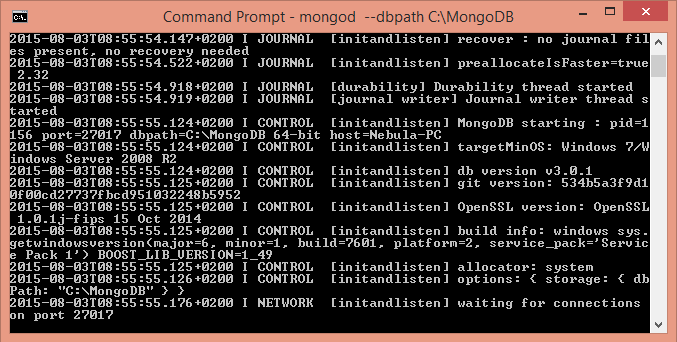
\includegraphics[width=1.0\textwidth]{screenshots/MongoDB.png}
    \caption{MongoDB Terminal - Expected output when running MongoDB} 
\end{figure}

Once mongo has been started, the CMS server can be started with the following command:\\ \\

\begin{verbatim}
~/Cafeteria_Management_System/$ grunt
\end{verbatim}

\begin{figure}[H]
  \centering
    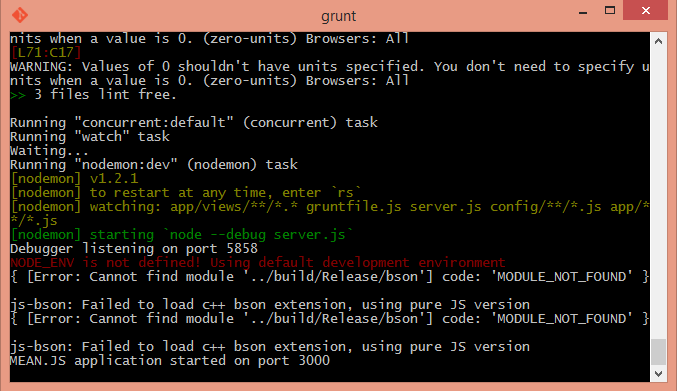
\includegraphics[width=1.0\textwidth]{screenshots/gruntOutput.png}
    \caption{Grunt - When grunt is running, output should be similar to this.} 
\end{figure}

Now the Server and the Database is running and we can get started with the rest of the setup process. \\
Note: Inside the browser one will run localhost:3000 to view  system. \\ 

To terminate the sever, the user can enter the Ctrl+C command in the terminal. The user can also terminate the MongoDB service by executing the same command (Ctrl+C) in the MongoDB terminal.

%%-------------------------------------GETTING STARTED ----------------------------------------
\section{Getting Started}
Access to the Cafeteria Management System is through a standard web browser. Different types of users have access to different facets of the system. The system has a default super user account and an admin user account which can assign different roles (cafeteria manager, cashier, etc.) to the users and which has global access to the whole system. These users can then sign in to access the facet of the system they are authorised to.\\

%%--------------------------------ADMINISTRATIVE USERS -------------------------
\subsection{Administrative Users}
When the CMS is started initially with an empty database there will be no users in the database this includes that there will  be no administrative users.  \\
Thus to generate the administrative users on the first startup of the system one shoud navigate to the sighn in page and sighn in with empty credentials. If the stystem is started for the first time with an empty database, on sighn in with empty credentials (this means click on the sighn in button without filling out the text boxes) administrative users will be created. \\

\textbf{The system will have a super user:} \\
Employee ID: SuperUser \\
Password: SuperUser \\

\textbf{And the system will also have an adminuser:} \\
Employee ID: AdminUser \\
Password: AdminUser \\

\textbf{WARNING :} \\
Administrative users will have global access to the whole system, thus it is of upmost importance that the administrative users should be set up with the first start up of the system and their credentials and passords must be changed to not violate the security of the system. \\ 

{\em* Note at all times there can only be 1 super user and 1 admin user - this is done for security purposes  } \\

Once logged in, the super user and admin user can change their password from the profile management page which is available directly from the home page. They can also set additional fields such as an e-mail address which will assist in password recovery in the event of a forgotten password and to where notifications about the CMS will be sent to.\\

%%-------------------------------- CREATING AN ACCOUNT -------------------------
\subsection{Creating an Account}
If you are a new user to the system you can create a new account by navigating to the Sign Up page by click the 'Sign Up' button on the navigation bar:

\begin{figure}[H]
  \centering
    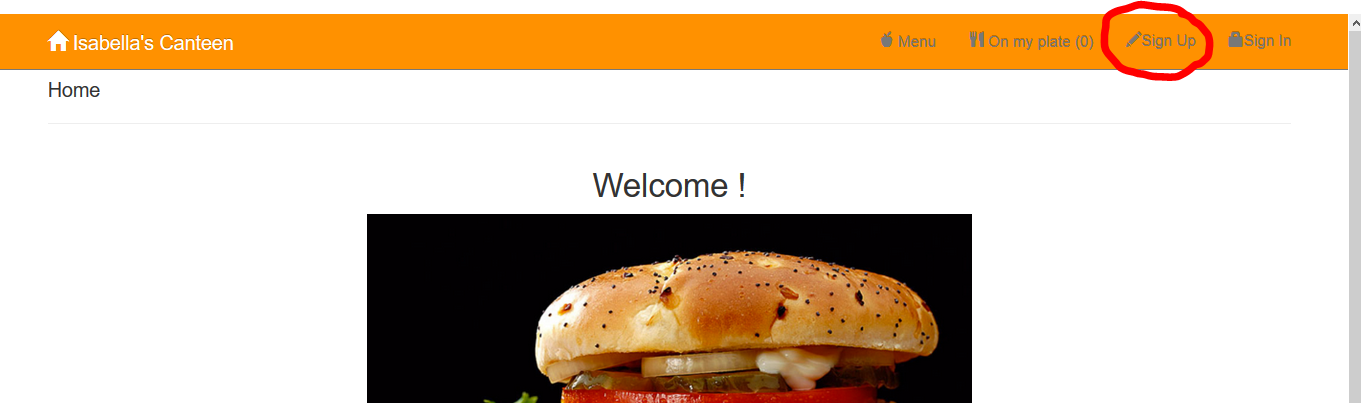
\includegraphics[width=1.0\textwidth]{screenshots/sighnUp.png}
    \caption{Sign-Up - red circled button should be clicked to sighn up} 
\end{figure}

When the button is clicked the CMS will rerirect you to the sighn up page where you can fill out all the details: \\

\begin{figure}[H]
  \centering
    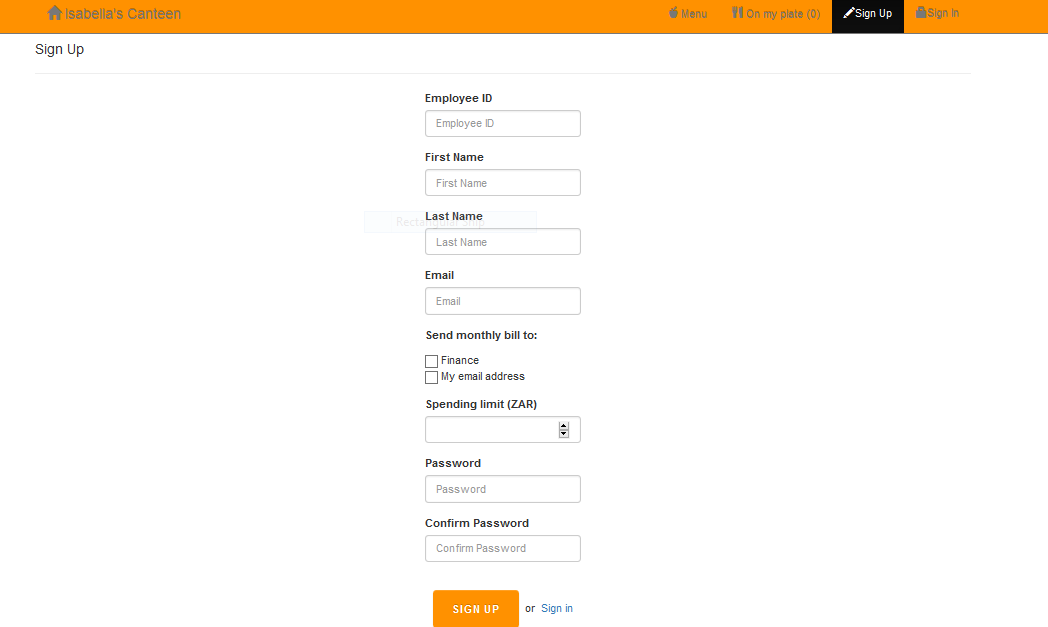
\includegraphics[width=1.0\textwidth]{screenshots/sighnUpPage.png}
    \caption{Sign-Up Page - detailes to be filled in - all fields are required} 
\end{figure}

{\em Employee ID } will be determined by the company where the cafeteria might find itself - no Employee ID can be reused.\\
The {\em e-mail address} is of importance for notifications when the order will be ready and for finantial bills to be send to. \\
The {\em spending} Limit is the maximum amount you may spend each month.\\

{\em Note that all the fields may be eddited when logged in} \\

After signing up and creating a new account the user will outomaticcally be logged in. \\

%%-------------------------------- LOGGING IN  -------------------------
\subsection{Logging In}
Once a user navigates to the home page of the CMS to log in the user can click on the button in the navigation bar called 'Sigh In':

\begin{figure}[H]
  \centering
    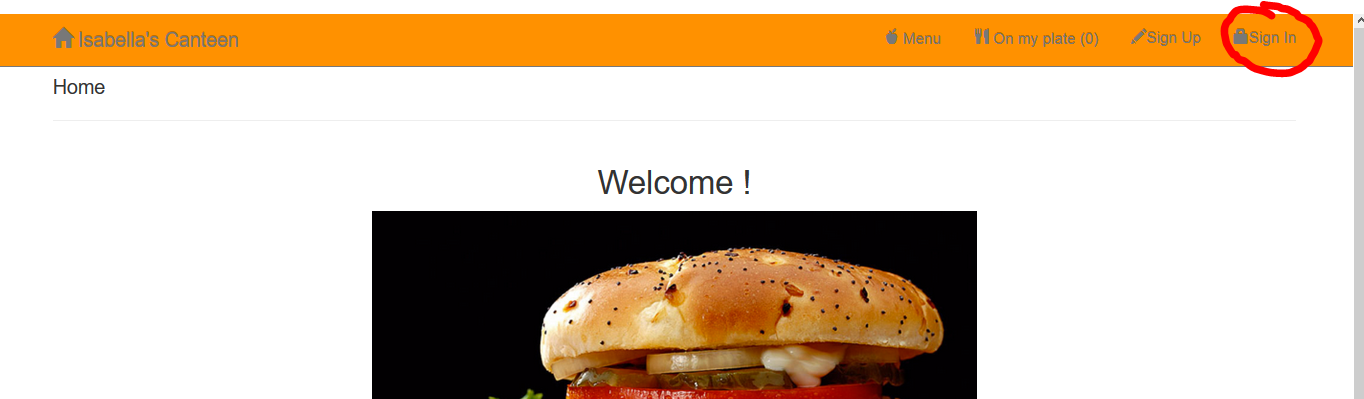
\includegraphics[width=1.0\textwidth]{screenshots/sighnIn.png}
    \caption{Sign - In - red circled button should be clicked to sighn in} 
\end{figure}

Once the user clicks on the sighn in button the CMS should direct to the sign in page :

\begin{figure}[H]
  \centering
    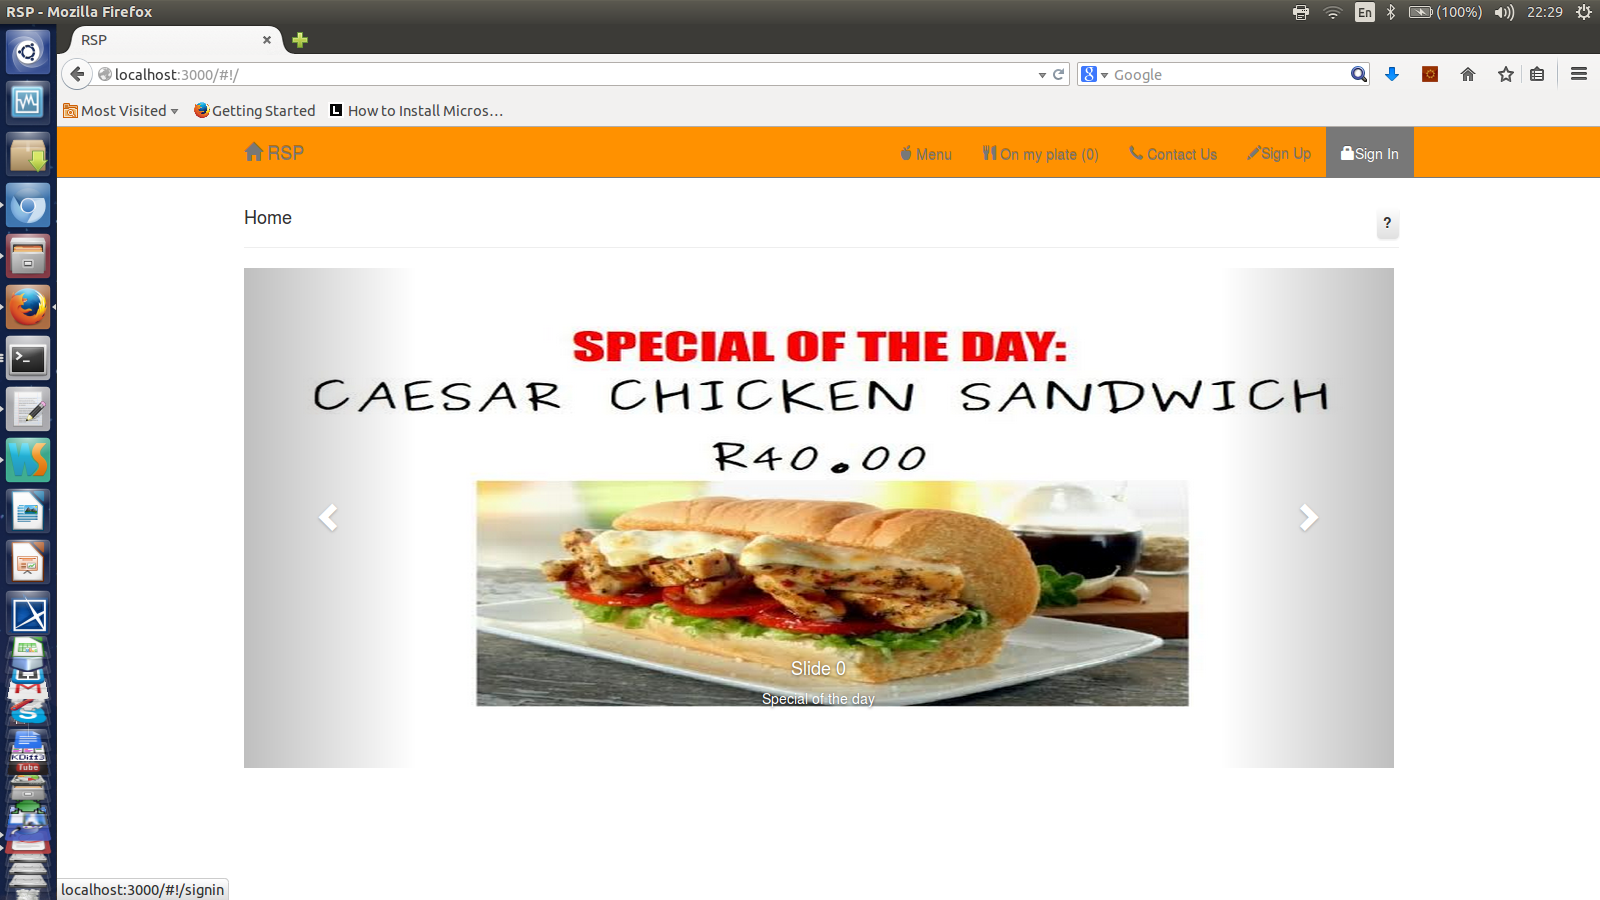
\includegraphics[width=1.0\textwidth]{screenshots/signIn.png}
    \caption{Sign - In page} 
\end{figure}

Only regestered users can sign in and fill out his/her personal details and click on the sign in button and the sustem will redirect to the home page when the user's login was sucessfull.\\
If the user can not log in due to forgetting his/her password they can click on the forget password link which will redirect to the forget password page:

\begin{figure}[H]
  \centering
    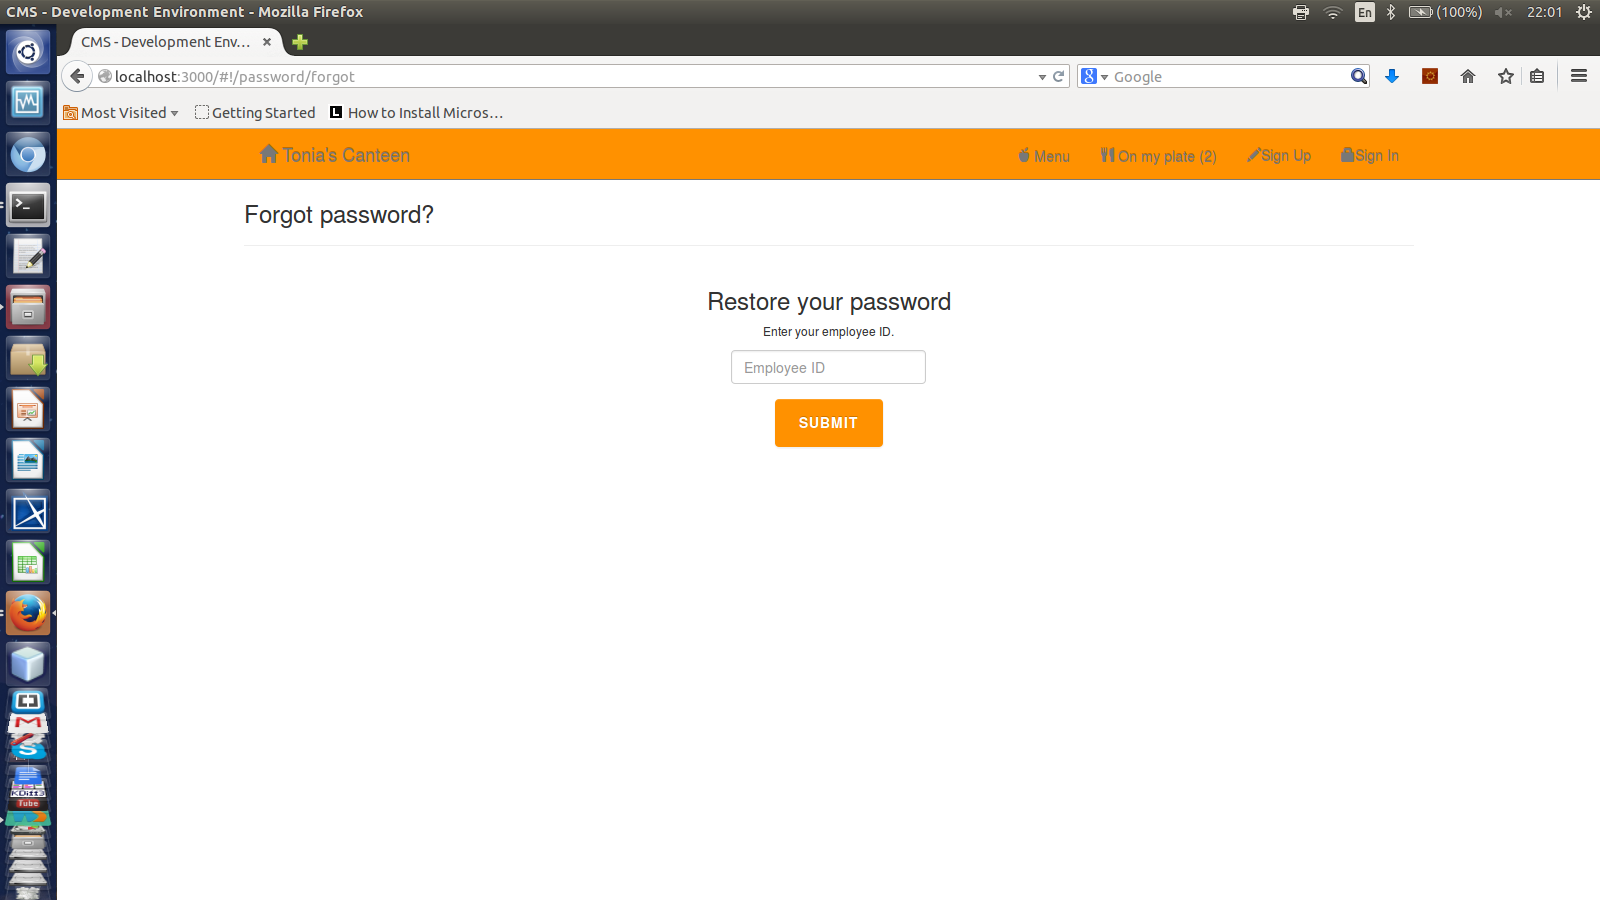
\includegraphics[width=1.0\textwidth]{screenshots/ForgotPass.png}
    \caption{Forgot password page} 
\end{figure}

The user can simply type in his/het Employee ID and click on the submit button, the CMS will send an e-mail notification to the user's registered e-mail address and he/she can just follow the link send by the CMS via e-mail and reset the password and try to log in again. \\

The rest of the functionality will be described in the section below in detail  under the respective headings of how to navigate between pages to administrative settings to ordering an item and so forth. 


%%-------------------------------------USING THE SYSTEM----------------------------------------
\section{Using The System} 
\subsection{The Navigation pane} 
The Navigation pane will when not logged in will be displayed as follows:

\begin{figure}[H]
  \centering
    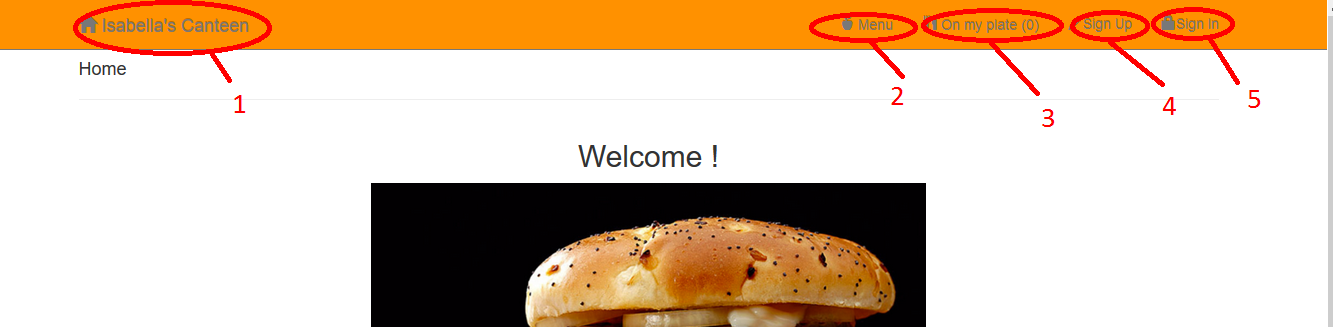
\includegraphics[width=1.0\textwidth]{screenshots/HomePage.png}
    \caption{Home Page - user not logged in } 
\end{figure}

The numbers in the images are described below:

\begin{enumerate}
\item The Home button - when clicking on this button it will always redirect to the home page
\item The Menu button - this button will redirect to the menui page
\item The on my plate button - this button will redirect to an orders page showing how many items you currently have on your plate and what they all consist of with totals.
\item The Sign Up button - this button will redirect to the sign up page where a new account can be created
\item The Sign In button - this button will redirect to a page where the usere can sign in and log into his/her account.
\end{enumerate}

On the home page, the name of the canteen is displayed. The user will also see the navigation pane at the top. The actions available with the pane are "Sign in", "Sign up", "Menu" and "On your plate". 
\\
The user can not proceed to order food if the user has not signed up and logged in. Hence, the first step a new user should take is signing up/ registering with the system. 
\\
If a user has not signed in, the user will still be allowed, however, to view the menu, without ordering anything. However, the user will be able to add items to their plate and view them on the "On My Plate" page, but the order will not be sent to the system until the user signs in.
\subsubsection{The Navigation pane - once the user has logged on}
The user will now view a drop down menu with various options displayed on it. The following options will be displayed if the user is a normal user: "Edit Profile", "Profile", "Sign out". These pages will be discussed below.
\\
If the user is a superuser the options "Admin Settings" and "Branding Settings" will be displayed. The superuser will hence be in control of assigning roles, changing employee ID's, setting the limit, changing the canteen name and the cover image of the canteen.  
\\
If the user is a cafeteria manager, the options "Manage Cafeteria" and "Manage Inventory" will be displayed. Manage Inventory is where the stock additions and removals are kept track of. Manage Cafeteria is where the different menu meal items will be logged.

If user is a financial manager, the option "Finance" will be displayed. The financial manager will be able to search for employees and view their bills, to keep track of these.

If the user is a cashier, the options "Placed Orders" will be displayed and it is here where the transactions will occur, such as marking whether orders are ready, and paid for. The cashier will also send notifications to the user, when the food is ready for the user to collect. 


\subsection{The "Sign Up" Page} 
Once the user has clicked the "Sign Up" option on the navigation pane, the user will be directed to the sing up form, where a user should fill in their details. Once completed, the user will click submit and if the form is correctly filled in the user will be notified upon success and will be signed up for the system. The user will hence be redirected to the home page. The user can then use the password created and employee ID to log in to the system. If the information entered is not followed, a thorough error message will be displayed indicating what the problem is so that the user can rectify it.
\\
The user must now log in to access the ordering and managing profile functionality.
\begin{figure}[H]
  \centering
    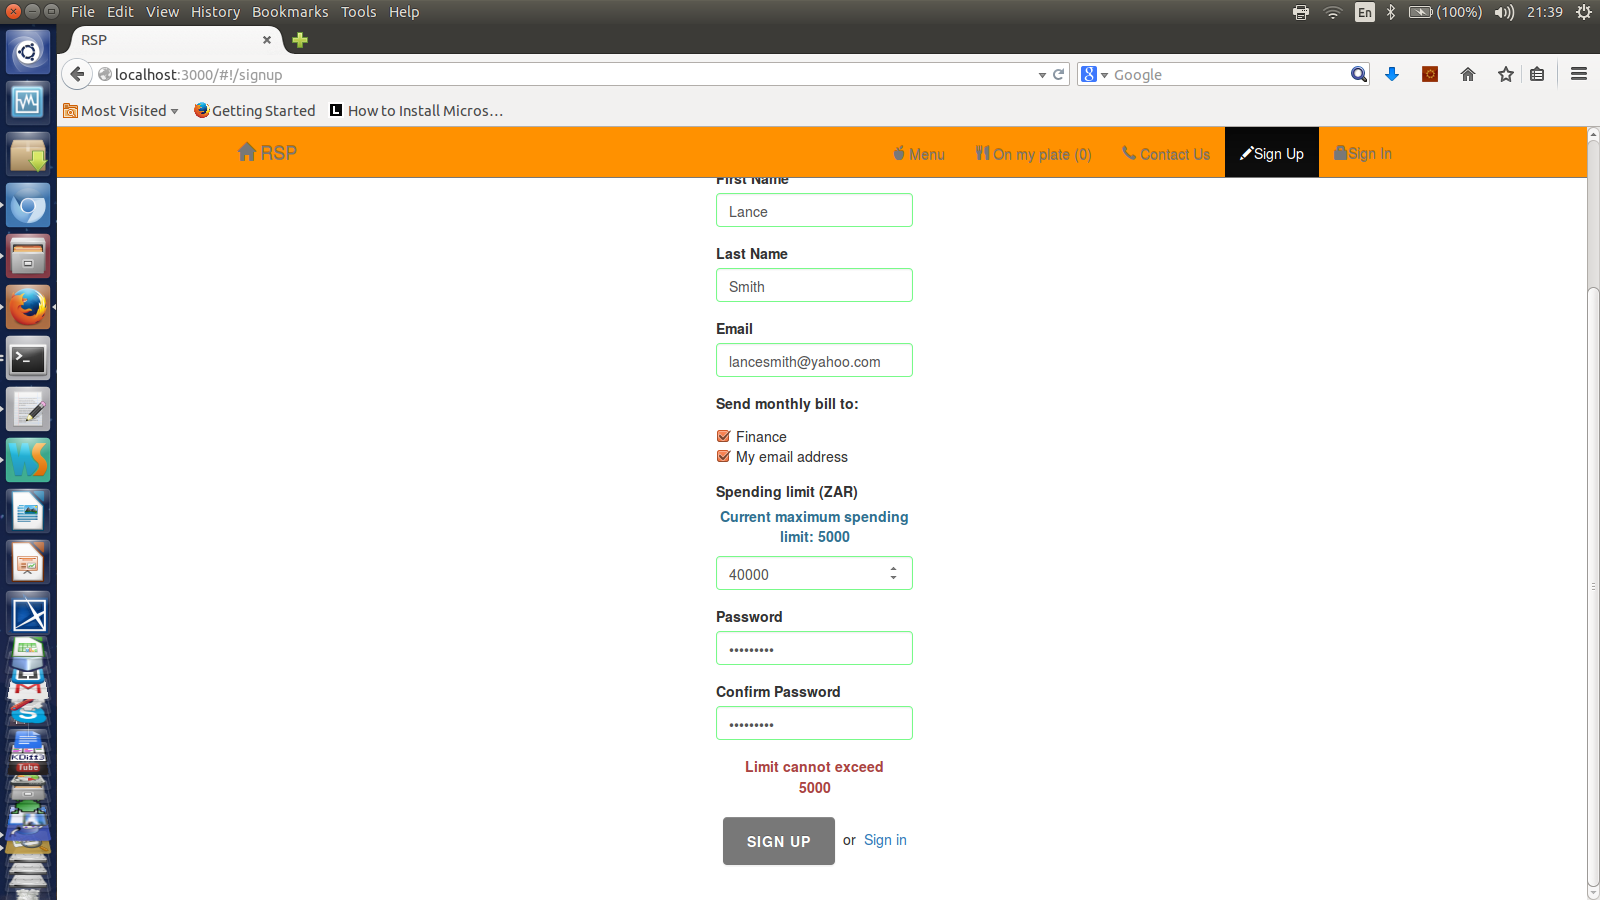
\includegraphics[width=1.0\textwidth]{screenshots/limitExeedSignUp.png}
    \caption{Sign up sheet - when a user types in a limit value larger than the maximum spending limit per month} 
\end{figure}

\subsection{The "Sign In" Page} 
To log into the system the user should click the Sign In option on the navigation pane. The user will fill in their password and Employee ID in the provided slots and click submit to proceed. If the information entered is valid, the user will be notified upon success and redirected to the home page, logged in on their personal account. If the information entered is not valid, a thorough error message will be displayed indicating what the problem is so that the user can rectify it.
\\
There is also an option called "Forgot your password?" which once clicked leads the user to a page where the user must enter their Employee ID. The user will then be notified that an email has been sent to their personal email account with further instructions on how to rectify the situation. The user will be sent a link to a page, in order to set a new password.   

\begin{figure}[H]
  \centering
    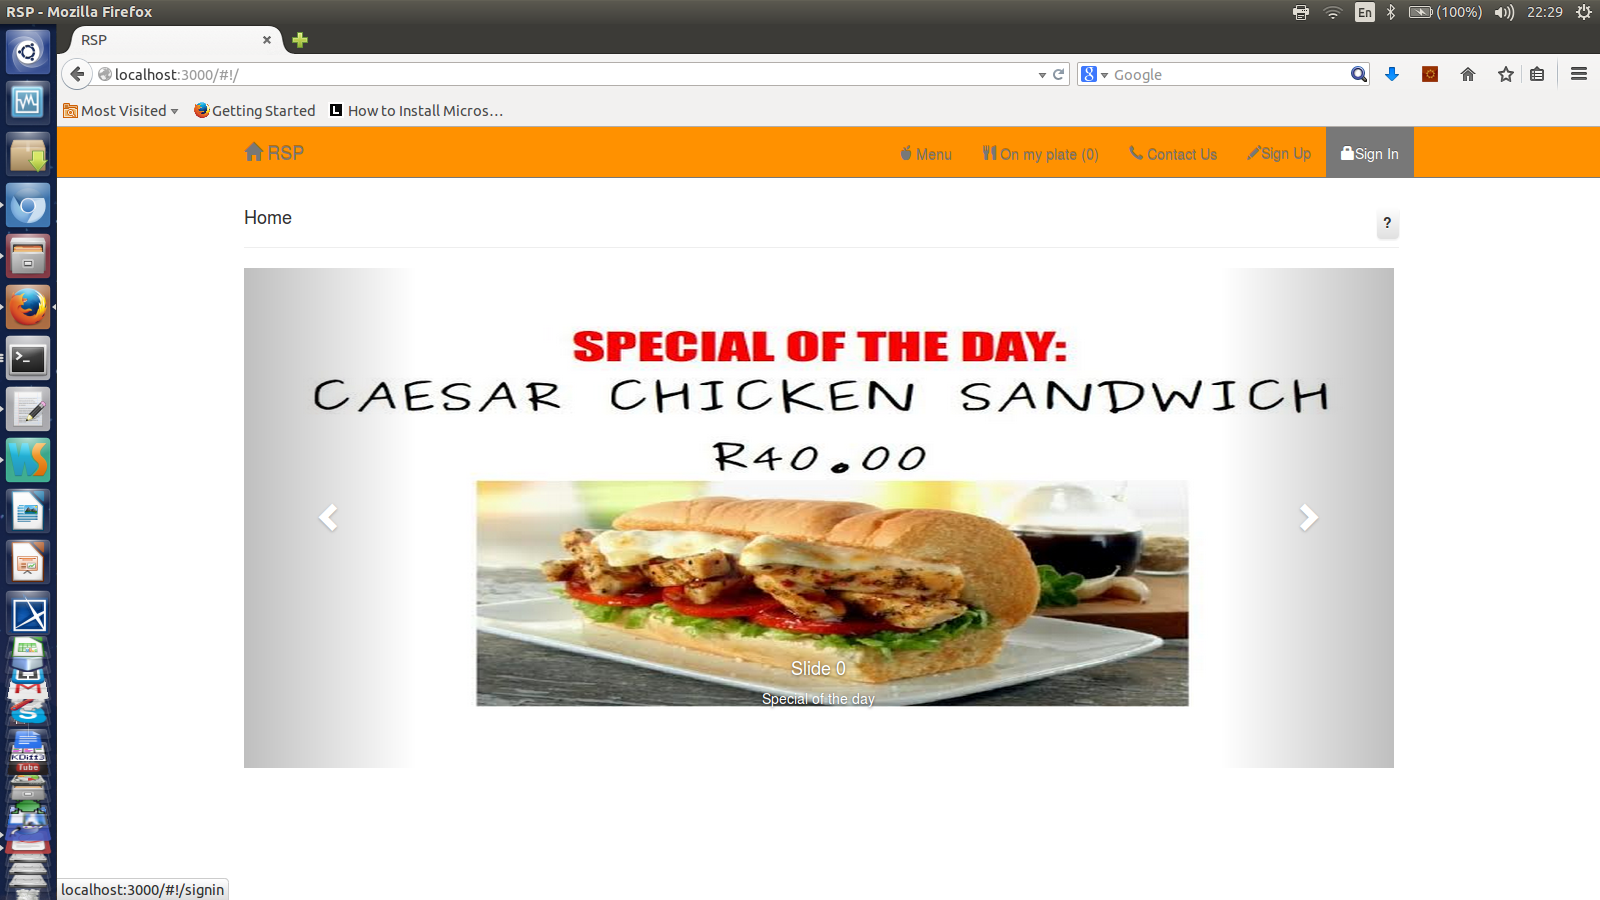
\includegraphics[width=1.0\textwidth]{screenshots/signIn.png}
    \caption{Sign In page - Type the appropriate information in the textboxes and click submit to sign in} 
\end{figure}

\begin{figure}[H]
  \centering
    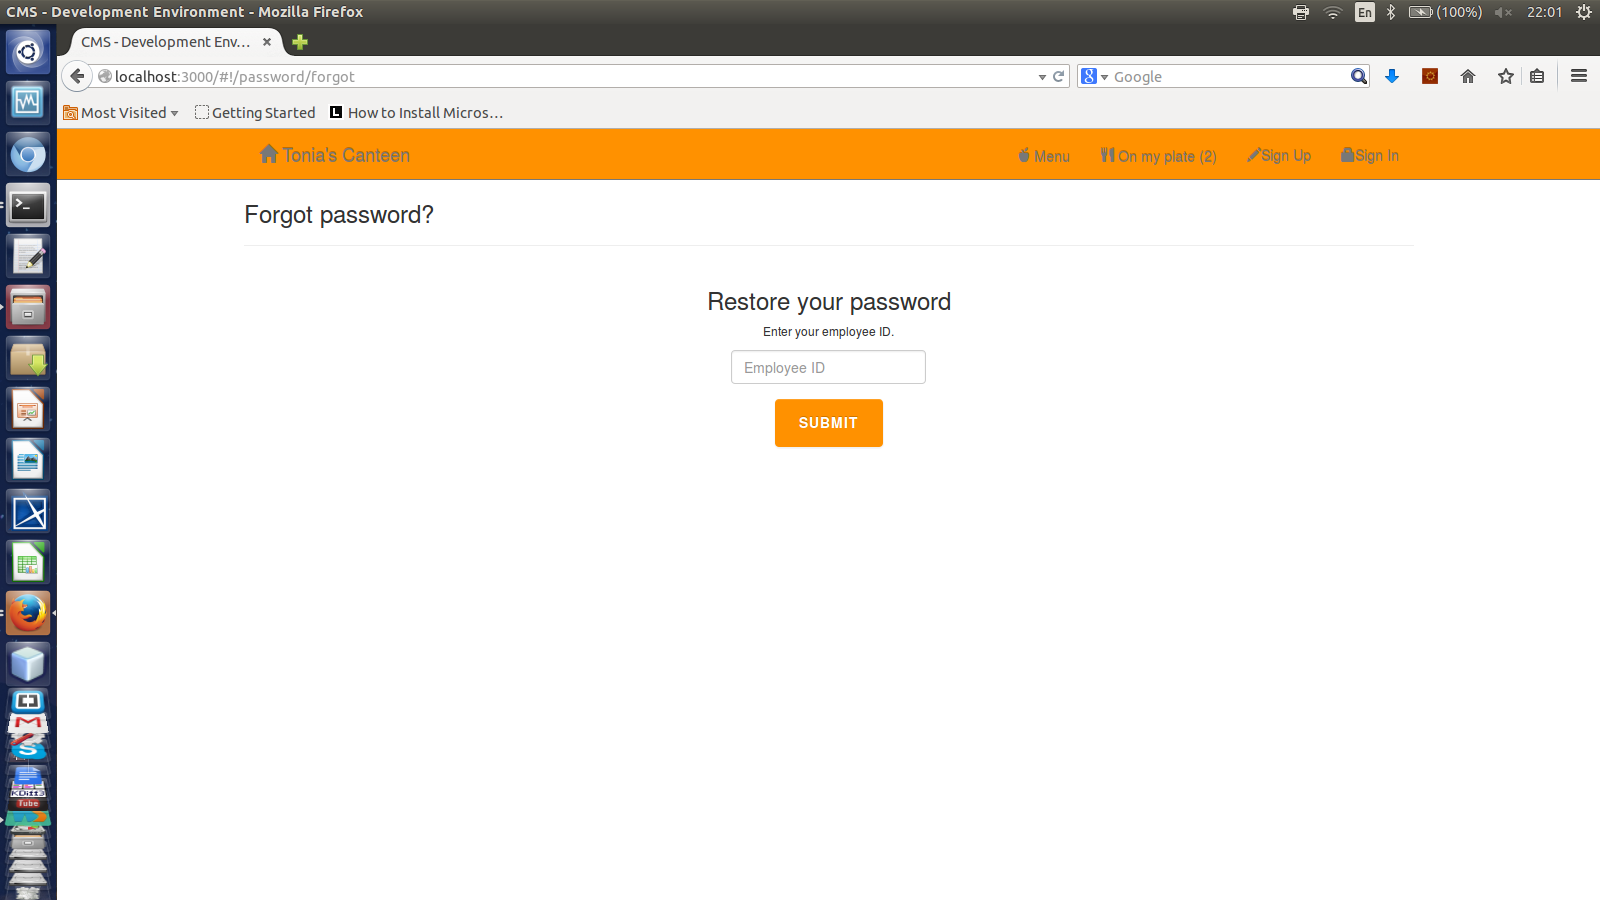
\includegraphics[width=1.0\textwidth]{screenshots/ForgotPass.png}
    \caption{Forgot password page} 
\end{figure}


\begin{figure}[H]
  \centering
    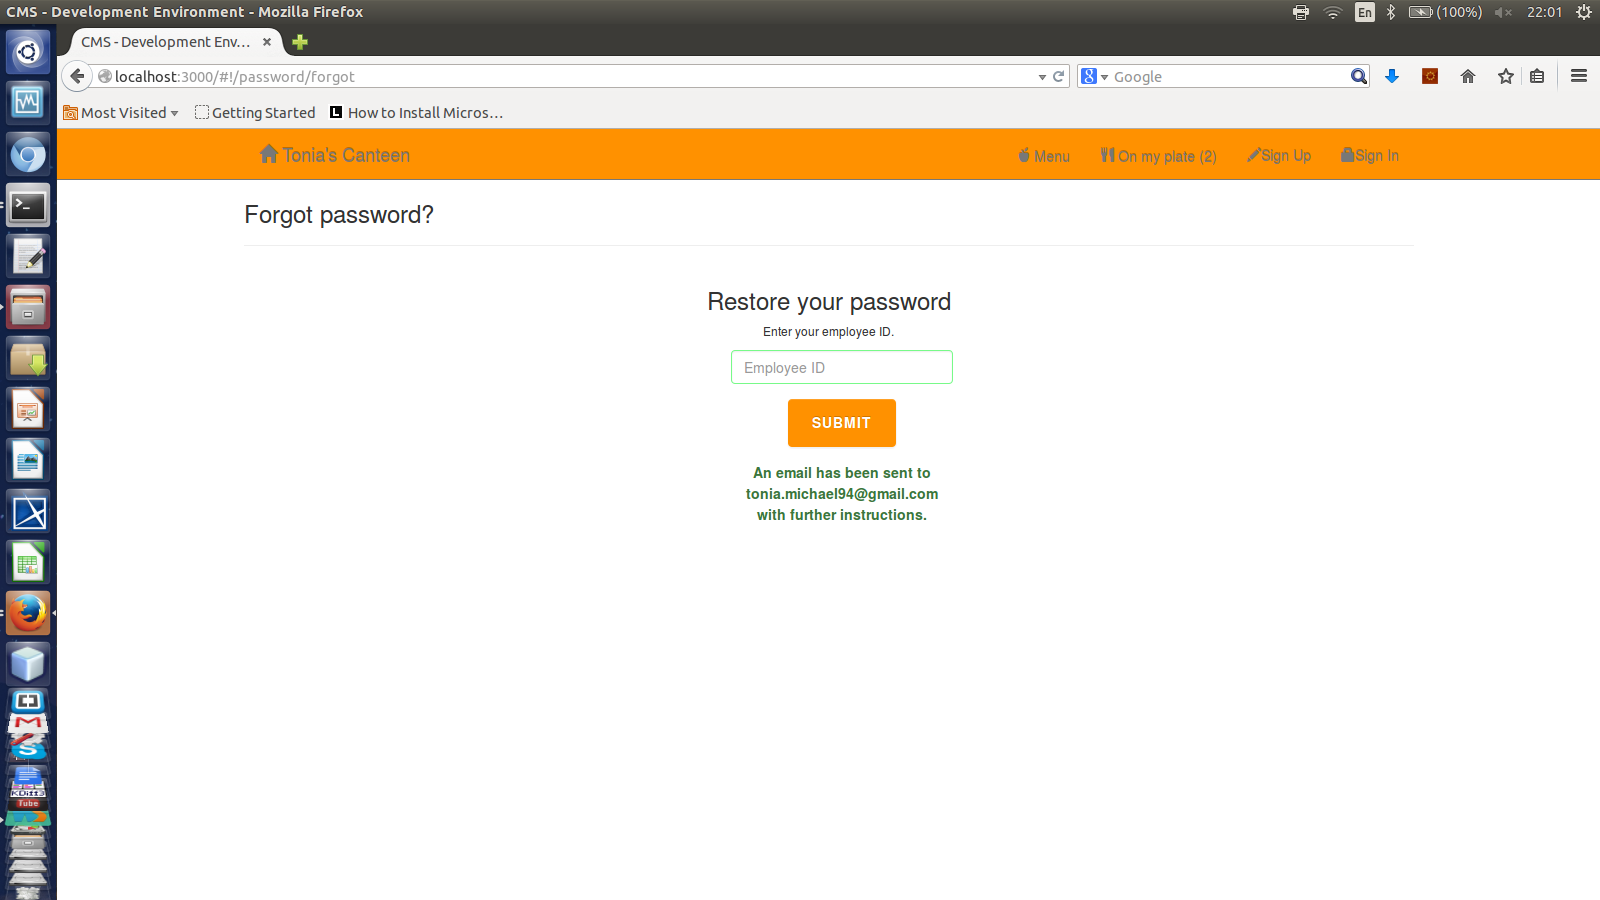
\includegraphics[width=1.0\textwidth]{screenshots/emailSentForPass.png}
    \caption{After submitting the form - notified about email sent} 
\end{figure}

\begin{figure}[H]
  \centering
    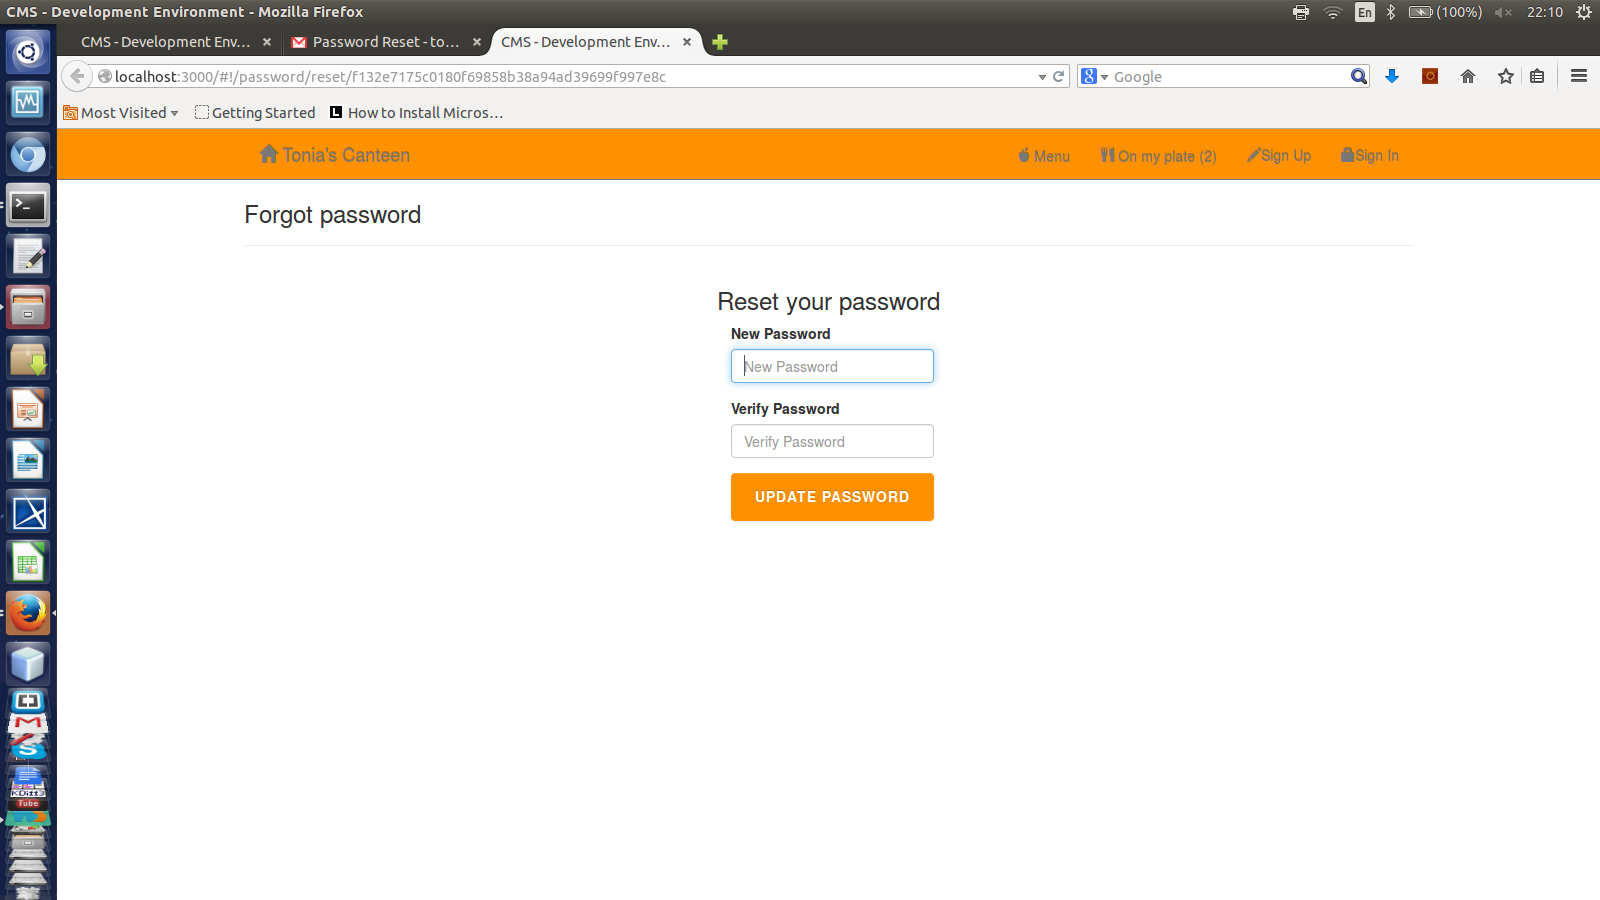
\includegraphics[width=1.0\textwidth]{screenshots/newPassForPass.png}
    \caption{The url sent via email leads to this page - fill in the textboxes and new password is set} 
\end{figure}

\subsection{The "Menu" Page} 
This is where the user will be able to view the menu items and their prices. An item can be added to the user's plate by simply clicking the 'Add to Plate' button alongside each item. These can then be viewed on the 'On my Plate' page.
\\
\begin{figure}[H]
  \centering
    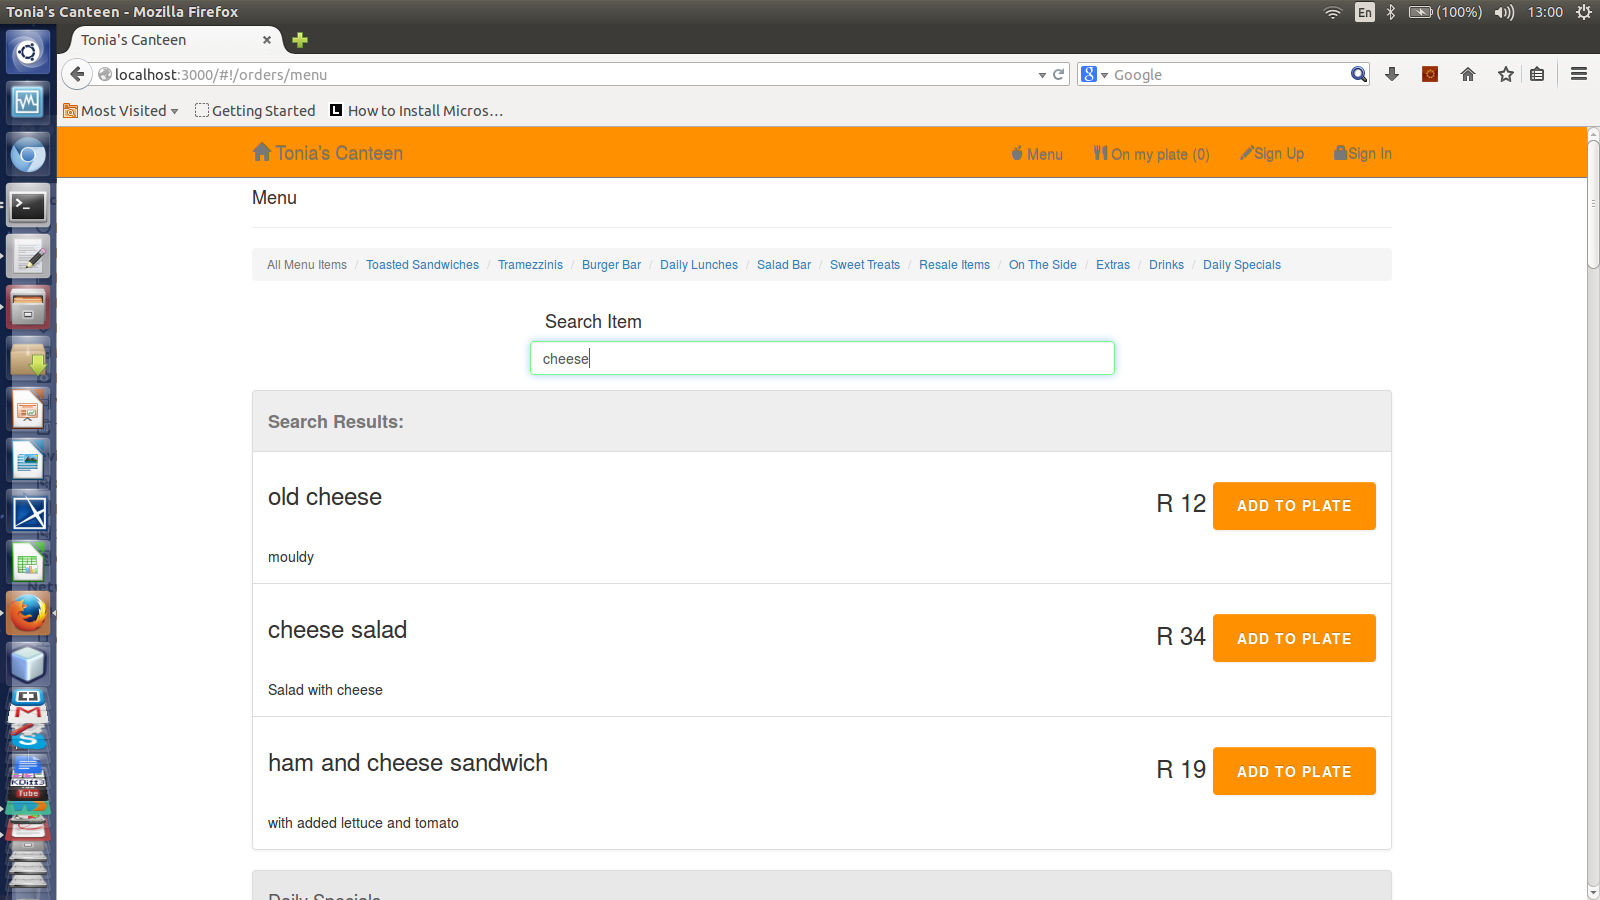
\includegraphics[width=1.0\textwidth]{screenshots/searchCheese.png}
    \caption{The menu page from which a user can order food} 
\end{figure}
On the menu page there is also a breadcrumb which indicates the different meal categories to make the search more efficient. There is also a search bar on all these pages. 

\begin{figure}[H]
  \centering
    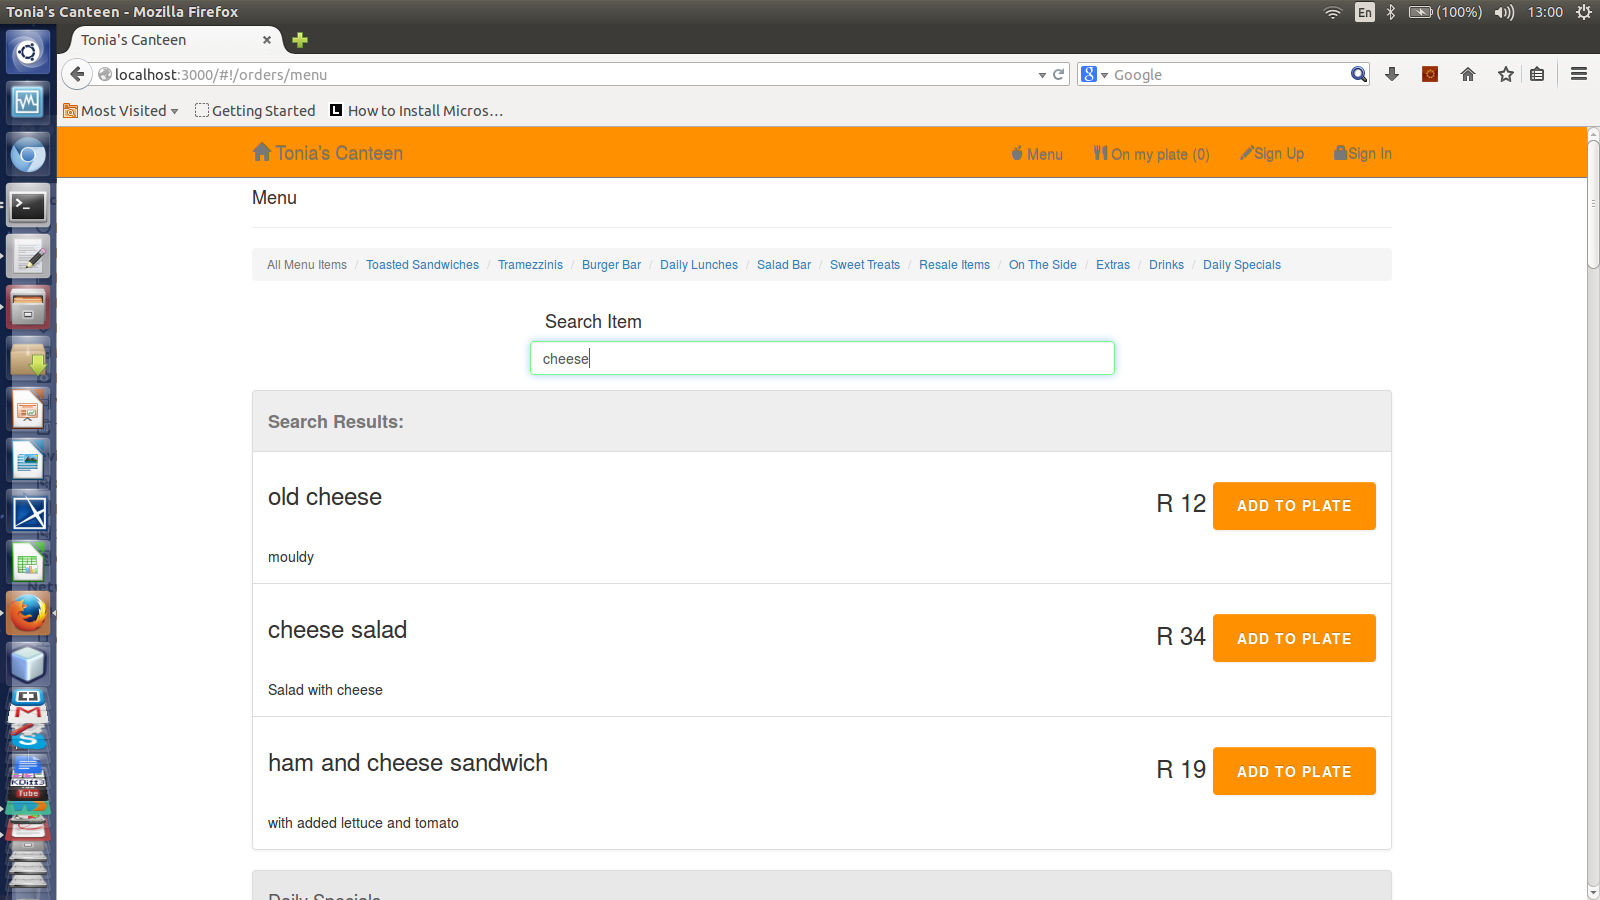
\includegraphics[width=1.0\textwidth]{screenshots/searchCheese.png}
    \caption{The menu page - Can be navigated via the search bar as illustrated} 
\end{figure}

\begin{figure}[H]
  \centering
    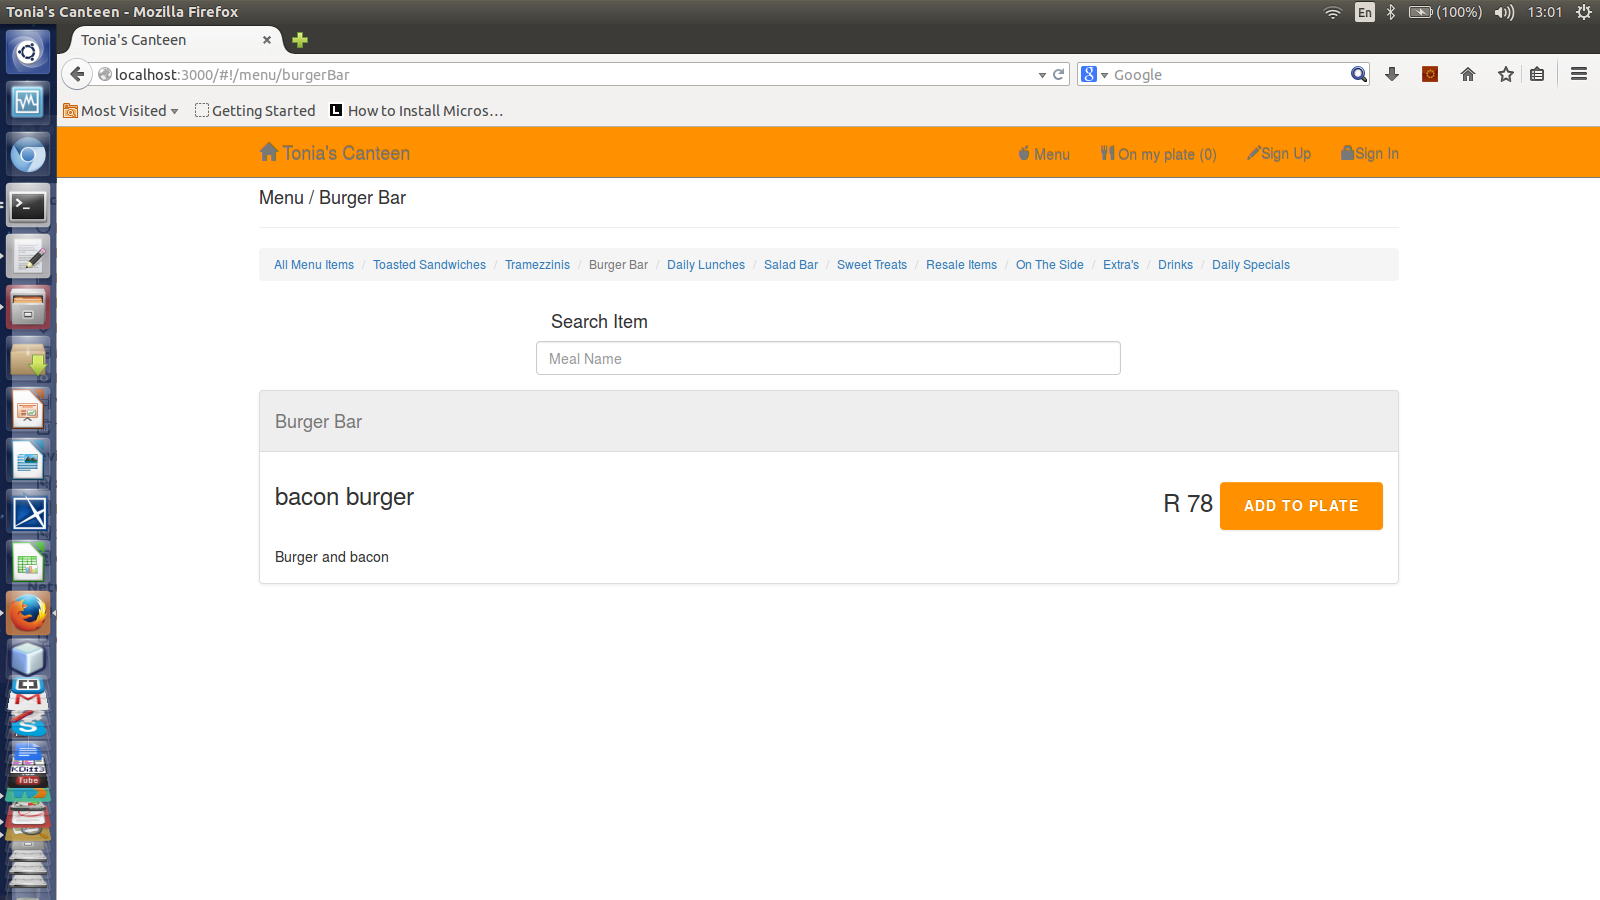
\includegraphics[width=1.0\textwidth]{screenshots/catMenu.png}
    \caption{The menu page - Can be navigated via the category breadcrumb as indicated to view sub menus} 
\end{figure}

\subsection{The "On my plate" Page} 
This page serves to indicate the current meal items that the user has ordered, and these can be removed on this page via the appropriately labelled button. The tab in the navigation bar also indicates an amount which is the amount of meal items ordered.


\begin{figure}[H]
  \centering
    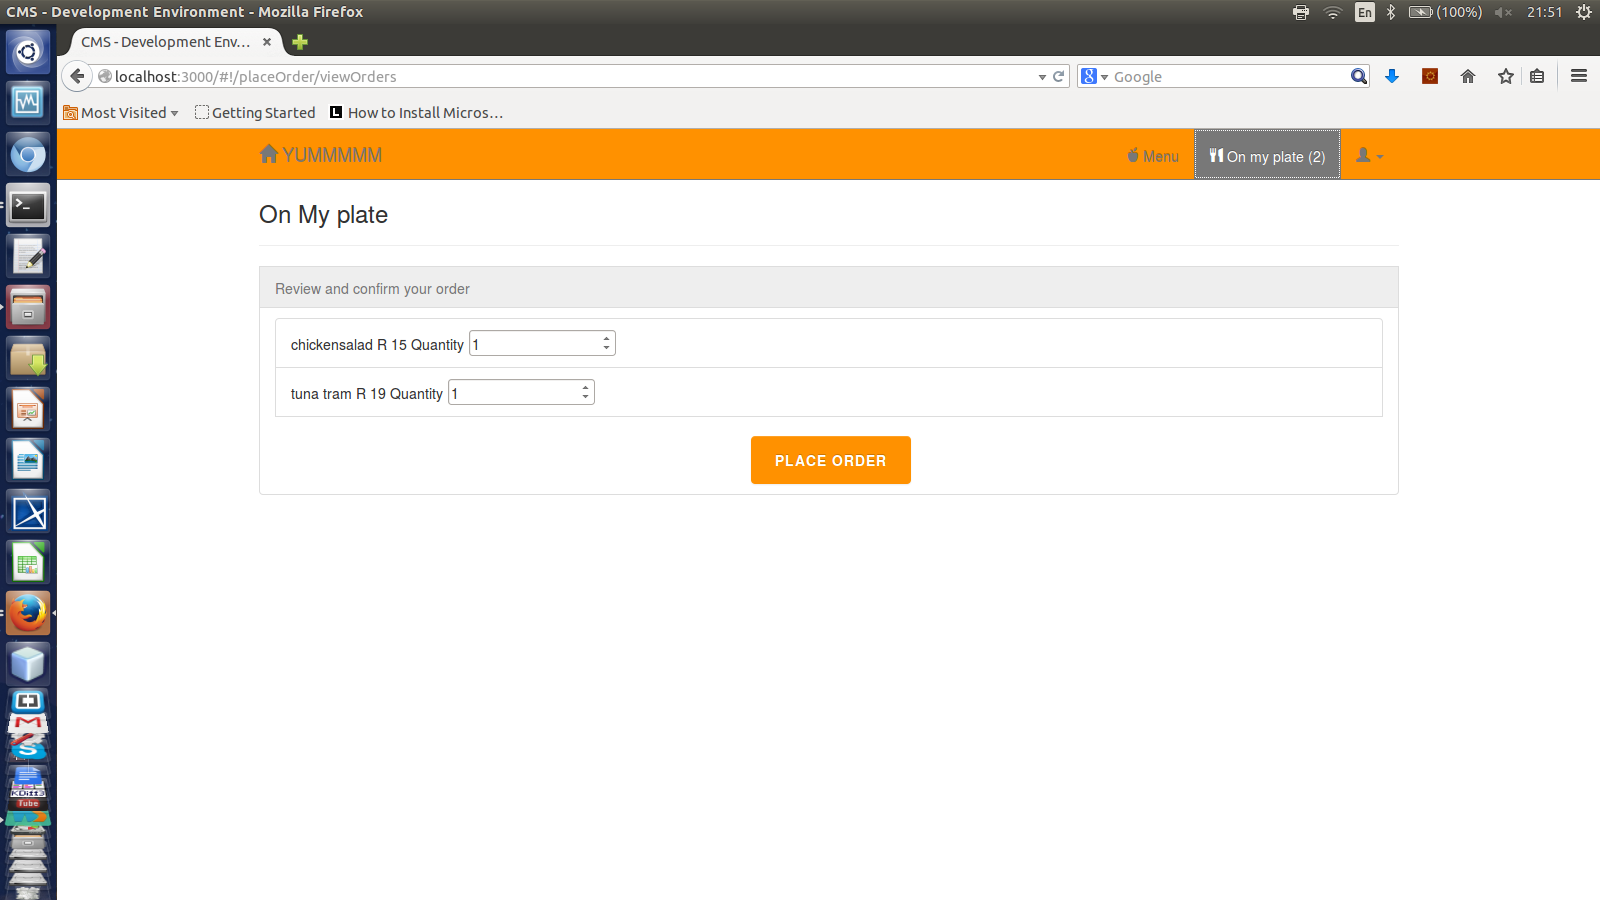
\includegraphics[width=1.0\textwidth]{screenshots/onPlate.png}
    \caption{On my plate page - The meal you selected on the menu page is displayed here (Navigate here via the navigation bar)} 
\end{figure}

\subsection{The "Edit Profile" Page} 
The user will be presented with a similar form to that which they signed up with, however, the details that the user entered in the sign up form will be present in these textboxes. The user can proceed to edit these here. Clicking the submit button will indicate whether changes have been saved or if errors have been made and how the user can correct these.

\begin{figure}[H]
  \centering
    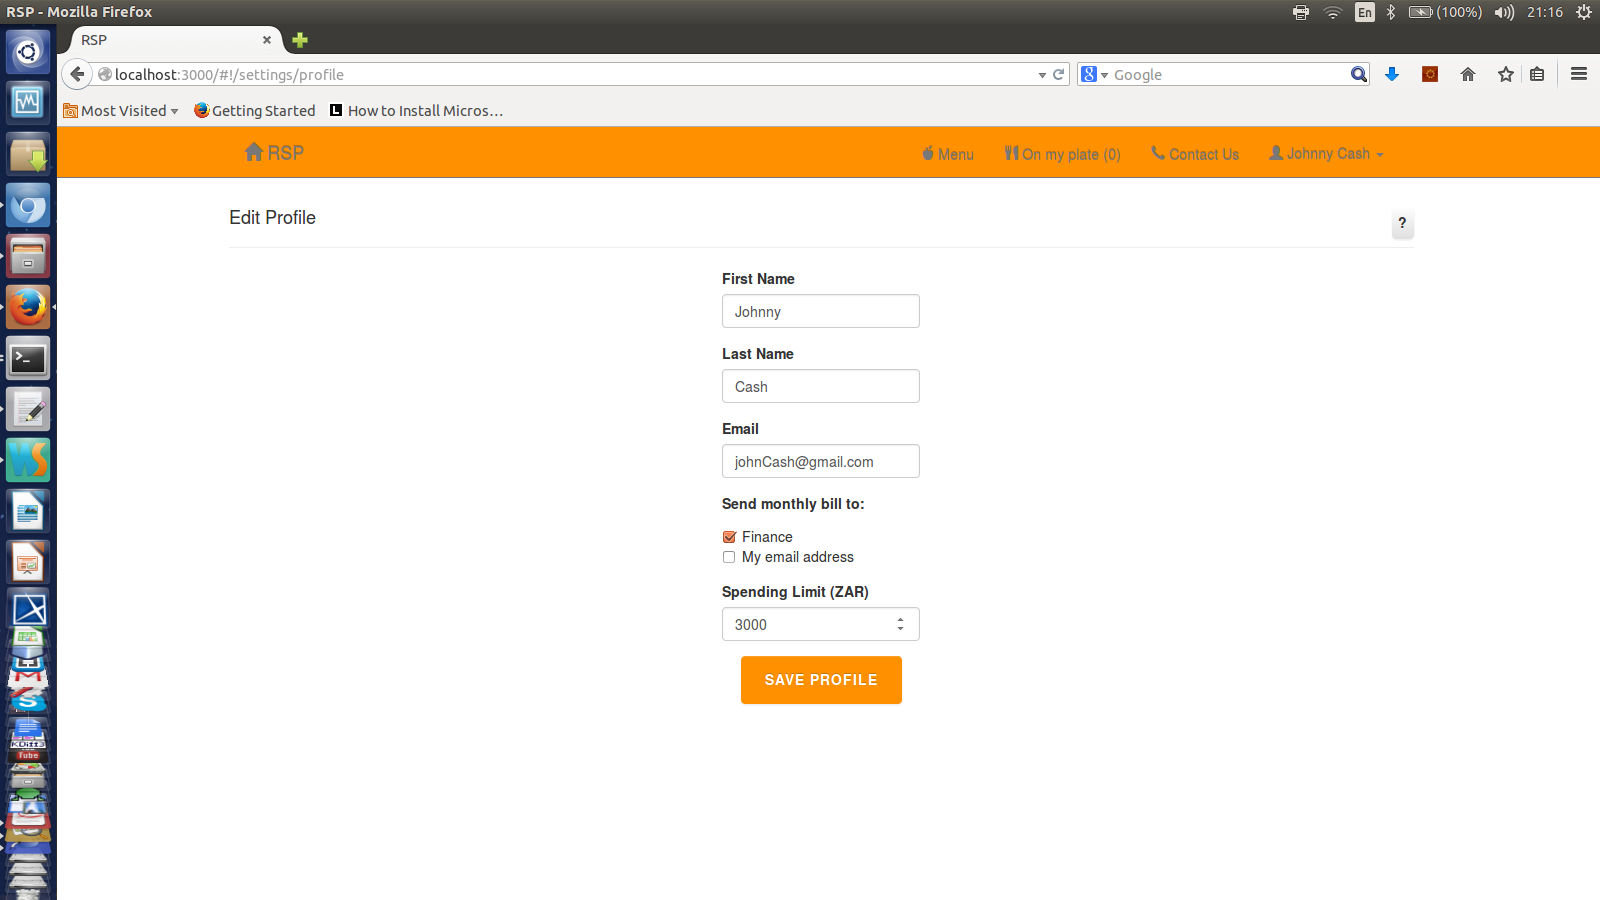
\includegraphics[width=1.0\textwidth]{screenshots/editProfile.png}
    \caption{Edit profile page - Edit profile by typing into the textboxes and submitting for validation message and to save new information } 
\end{figure}

\begin{figure}[H]
  \centering
    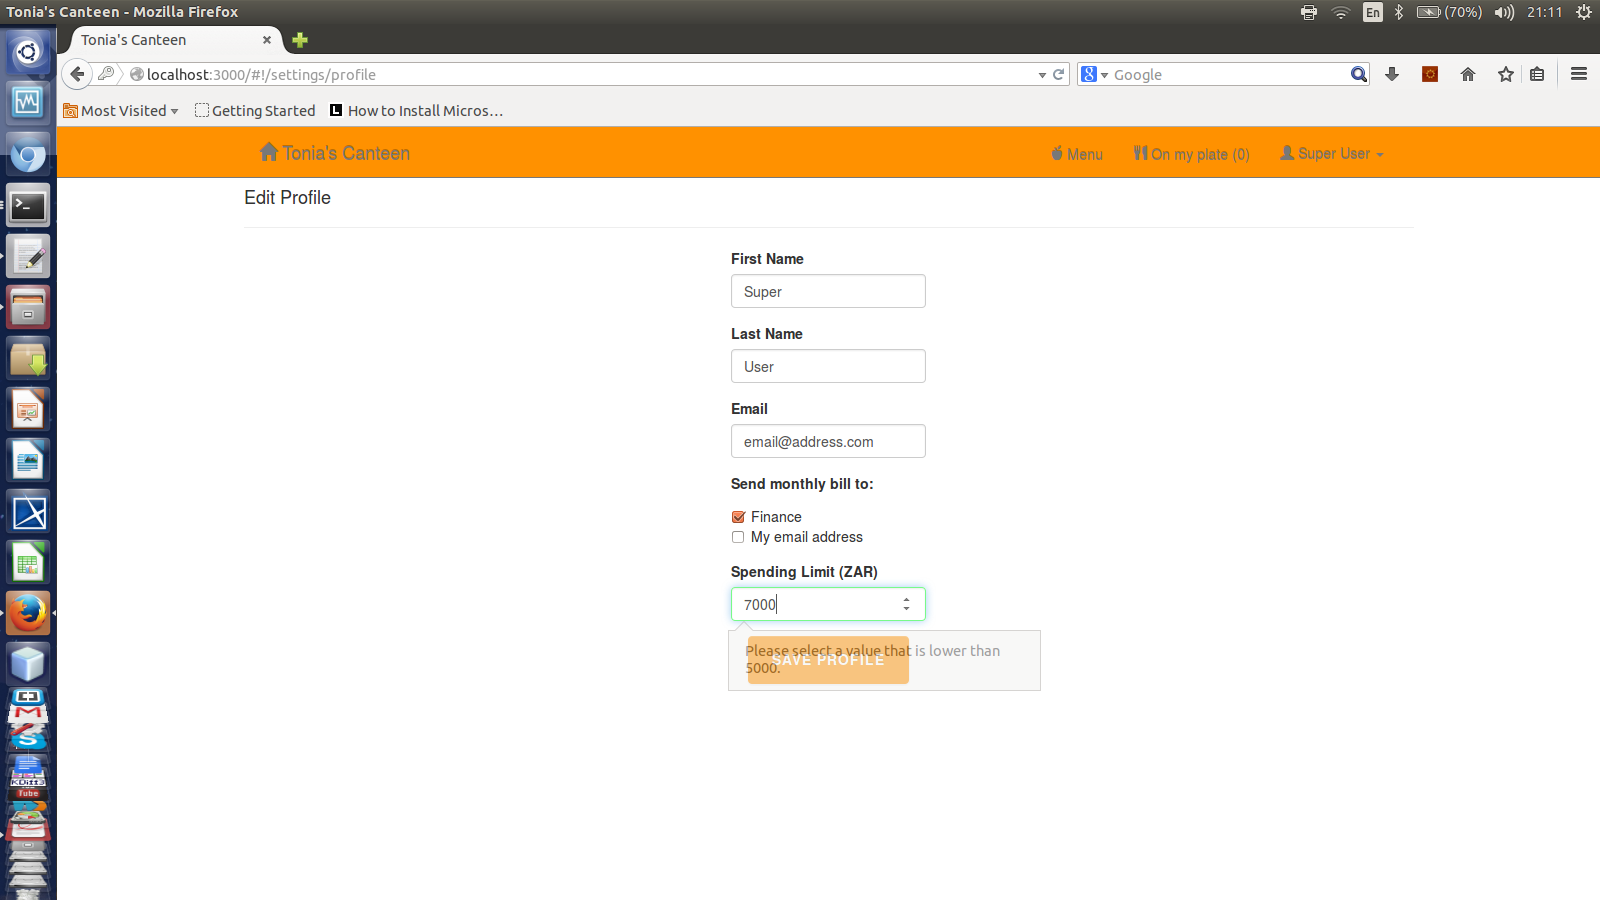
\includegraphics[width=1.0\textwidth]{screenshots/limitExeeds.png}
    \caption{You must ensure your monthly spending limit is within the bounds of the maximum spending limit of the system, set by the superuser} 
\end{figure}

\subsection{The "Profile" Page} 
This is where the user will be able to view their profile i.e. the details they entered when they signed up/ edited their profile. 

\begin{figure}[H]
  \centering
    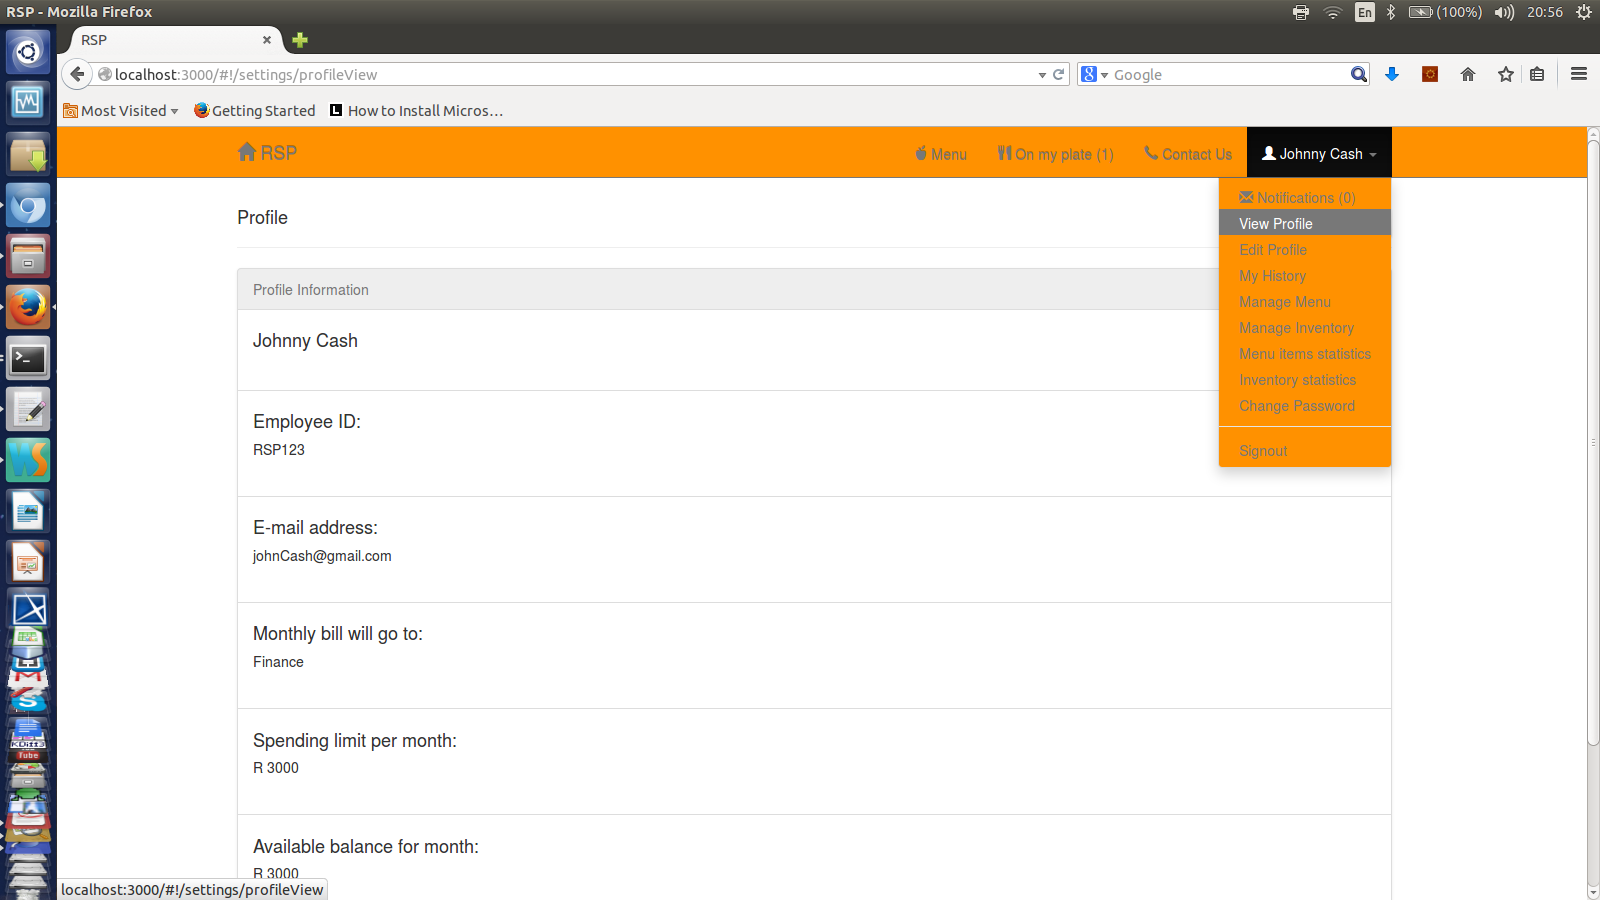
\includegraphics[width=1.0\textwidth]{screenshots/viewProfile.png}
    \caption{The profile page - where you view your profile (via the orange navigation tab menu indicated)} 
\end{figure}

\subsection{The "Change Password" Page} 
The user is presented with a form where the user will be asked to enter their old and new passwords to change their password. 

\begin{figure}[H]
  \centering
    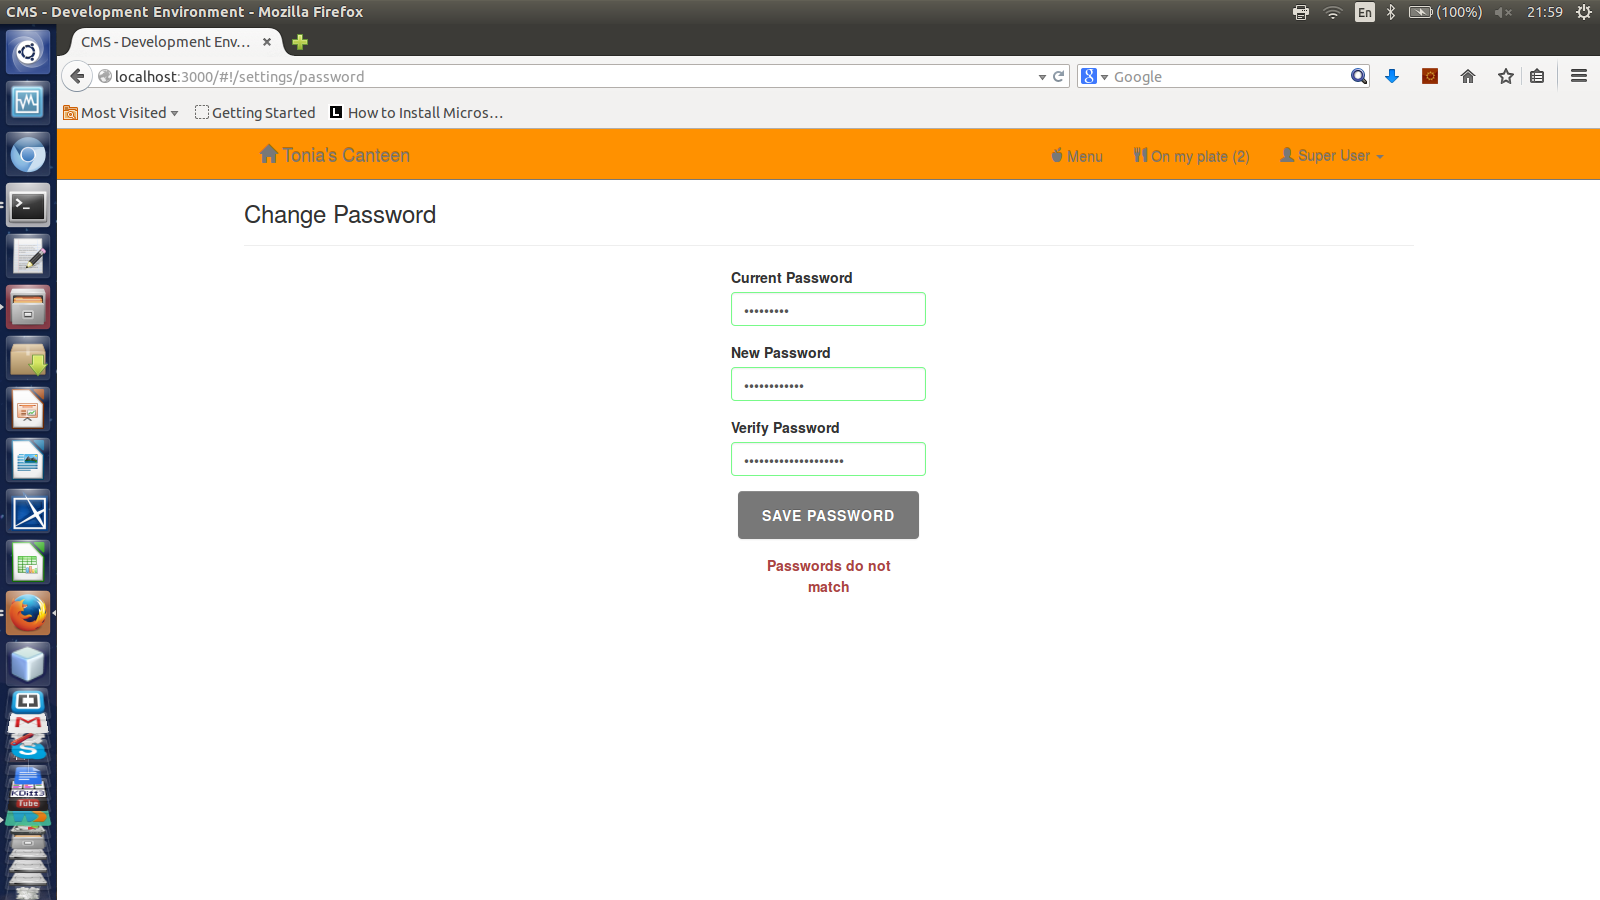
\includegraphics[width=1.0\textwidth]{screenshots/changePassDontMatch.png}
    \caption{Can change password on this page - validation message will be displayed indicating if change was successful or not} 
\end{figure}

\subsection{Superuser: The "Administrative Settings" Page} 
At the top of the page there is a section labelled assign roles, where different admin roles will be assigned to different users. The superuser simply has to type in an employee ID and select a role from the dropdown menu below. There is a section underneath that where the superuser can change the user ID of an employee. Self explanatory textboxes are provided for the superuser to fill in and the submit button will save the changes, unless an error occurs.  This page also consists of a section labelled "Change system limit" and it is here where the superuser can alter the limit of the system, i.e. the maximum value that a user can set their daily spending limits to. Hence a textbox is provided for the superuser to type the new limit and save it.

\begin{figure}[H]
  \centering
    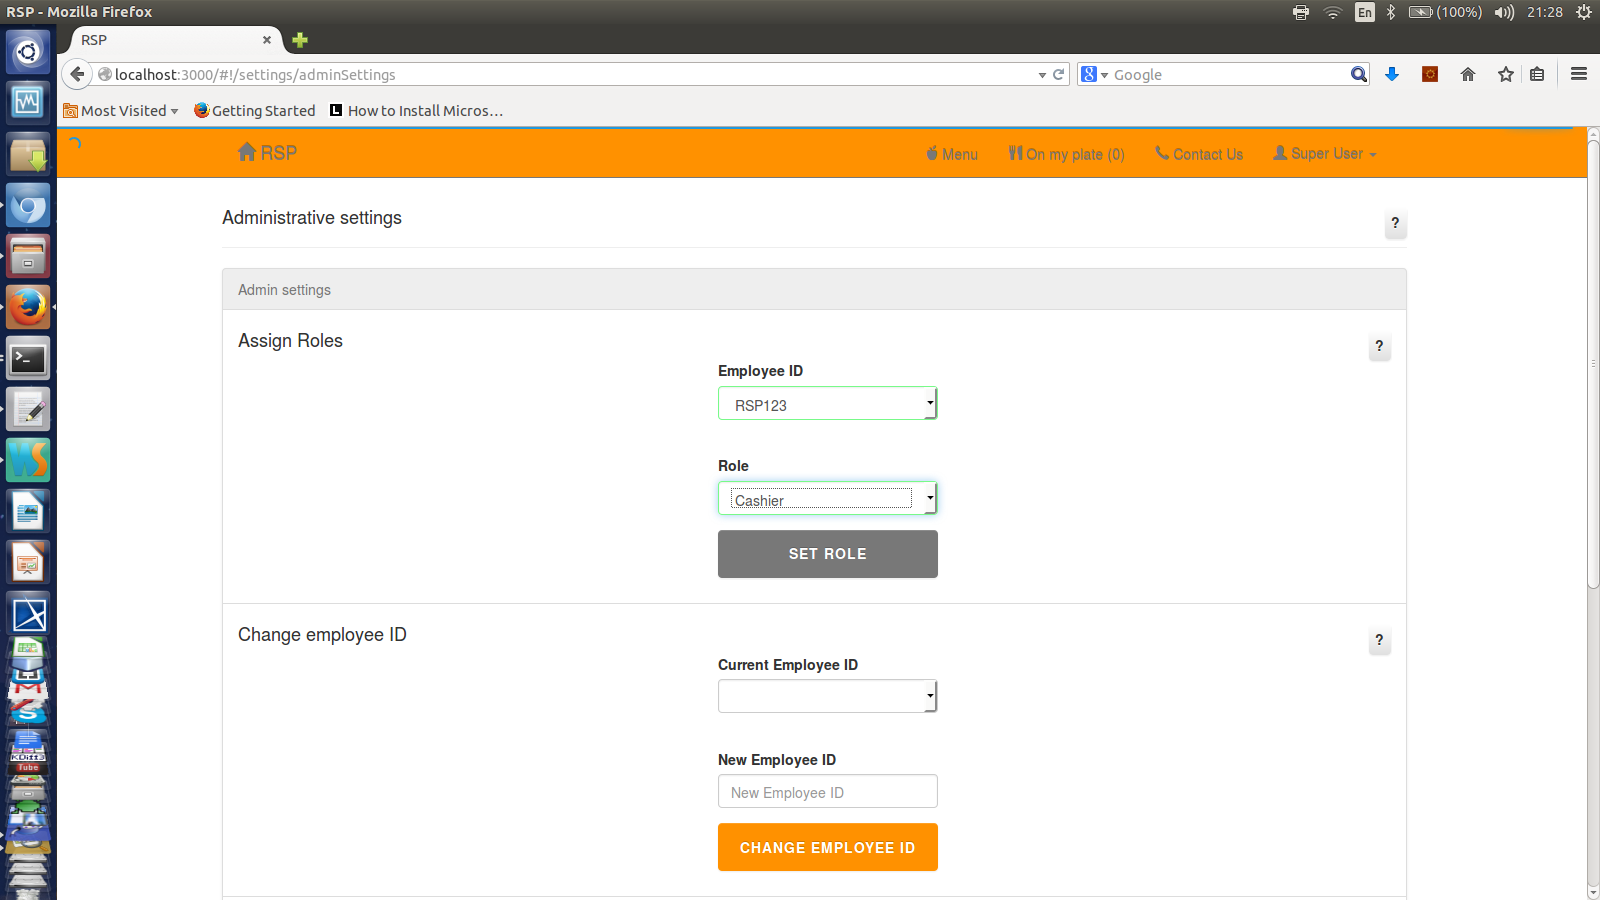
\includegraphics[width=1.0\textwidth]{screenshots/assignRole.png}
    \caption{The admin page - superuser can assign roles such as cashier to users} 
\end{figure}

\subsection{Superuser: The "Branding Settings" Page} 
There are two sections on this page. One where the user can change the canteen name, by merely typing in a new name over the old name in the allocated textbox, and another where the superuser can upload a new cover photo for the system.

\begin{figure}[H]
  \centering
    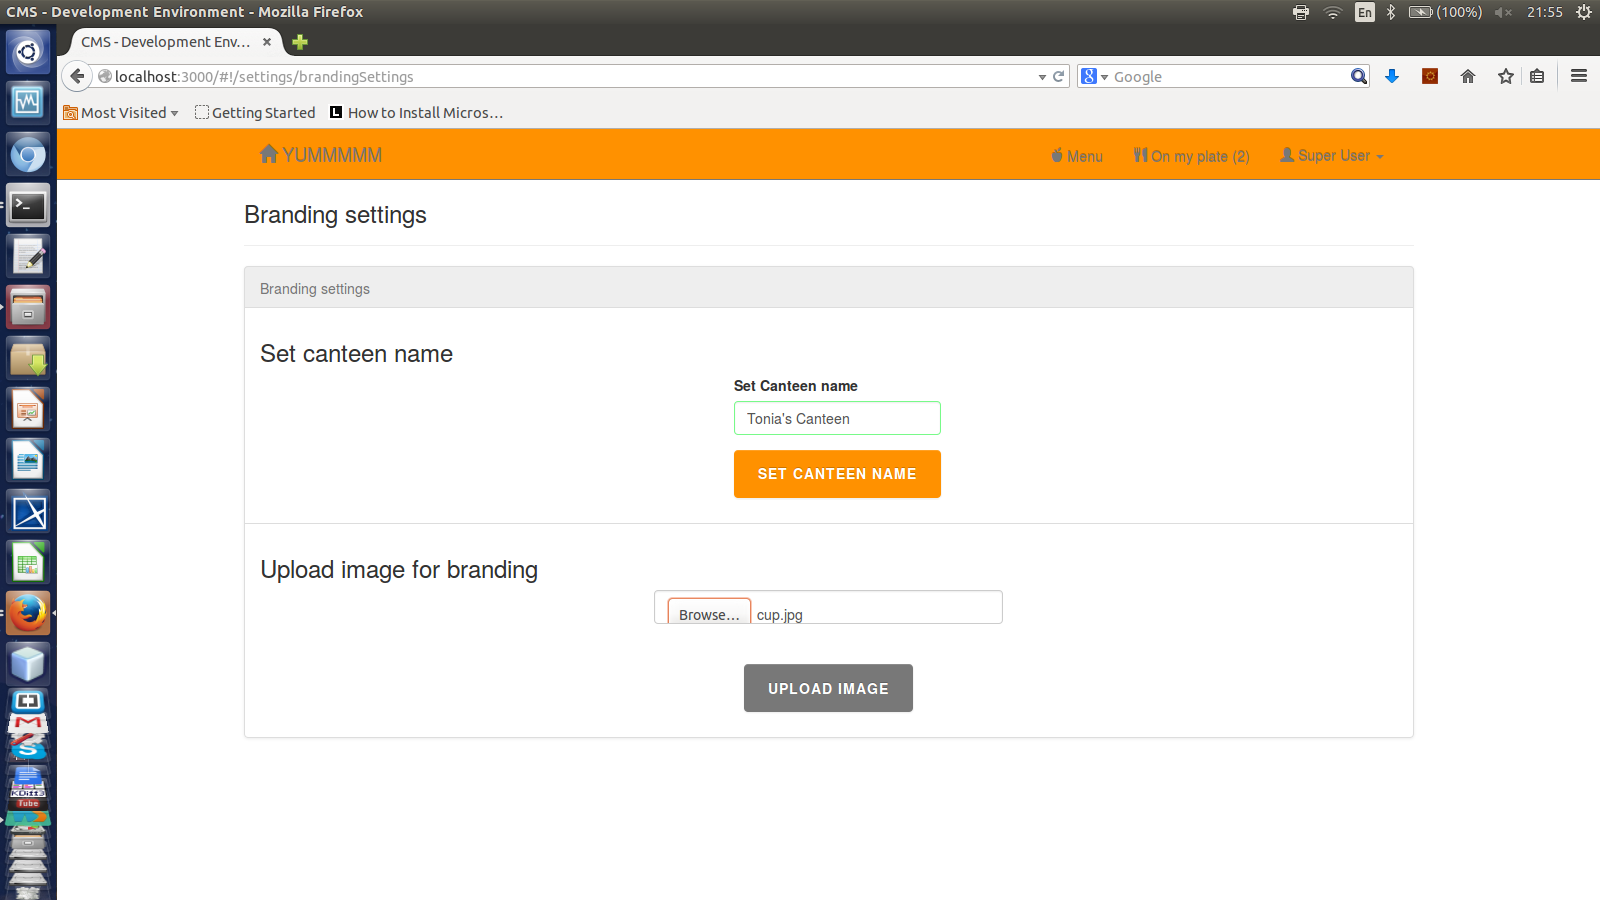
\includegraphics[width=1.0\textwidth]{screenshots/coverImage.png}
    \caption{The admin settings page - superuser can change the System Branding} 
\end{figure}

\subsection{Cashier: The "Process Orders" Page}
This page is for the use of the cashier. Orders can be marked as ready via the checkboxes and can also be marked as completed or paid and completed. The option "Send notification" is available for the cashier to send an email to the users when their order is ready for collection.

\subsection{Financial Manager: The "View Employee Bills" Page}
There is a field labelled "Employee Id" and it is in here where a user will type in the employee ID 

\section{Troubleshooting}
\subsection{Problems with setting up the system}
If the system does not start up when you run the 'grunt' command, either of the following procedures can be followed:
\begin{itemize}
\item Ensure you have an active internet connection as the system requires an internet connection.
\item Ensure you have MongoDB running in a separate terminal. \\
	The line \begin{verbatim}
		Waiting for connections on port 27017
	\end{verbatim} should be displayed at the end of the Mongo terminal.
\item If the above does not solve the problem, the command npm update should be run from inside the CMS directory:
	\begin{verbatim}
		~/Cafeteria Management System$ npm update
	\end{verbatim}
\item If the problem persists the following commands should be run in order:
	\begin{verbatim}
		~/Cafeteria Management System$ bower install
	\end{verbatim} 
	\begin{verbatim}
		~/Cafeteria Management System$ npm install
	\end{verbatim} 
	\begin{verbatim}
		~/Cafeteria Management System$ npm update
	\end{verbatim}
\end{itemize}

%%-------------------SUPPORTING DOCUMENTATION -----------------------------
\section{Other Supporting Documentation}

For other supporting documentation regarding the CMS please refer to the GitHub repository: \\

 \url{https://github.com/toniamichael94/MainProjectCOS301}
\end{document}